\hypertarget{ch4}{%
\chapter{Comparing multisensor optical-radar approaches for snow water equivalent retrievals}\label{ch4}}

%==============================================================================
%=============================================================================
%==============================================================================

\hypertarget{ch4-abstract}{\section{Abstract}\label{ch4-abstract}}
For several decades, satellite remote sensing has been a valuable tool for mapping snow cover globally, regionally, and locally. However, no remote sensing technique can accurately measure snow water equivalent (SWE) from space for mountain hydrologic applications. Optical sensors like MODIS, VIIRS, and Landsat are robust for measuring the fractional snow-covered area (fSCA) at various spatial and temporal resolutions. Yet, these optical methods are limited by cloud cover and do not provide information on SWE. Synthetic aperture radar (SAR) can penetrate clouds, has a fine spatial resolution, and various algorithms allow us to quantify both SWE magnitude and changes. While SAR-based techniques show promise for SWE monitoring, they cannot discriminate between snow-free and snow-covered areas when the snow is dry. To address this SWE monitoring challenge, we evaluate a multisensor approach that leverages the strengths of both optical and radar sensors. Our study aims to better understand the variability between common snow cover data products and how that uncertainty propagates into InSAR-based SWE retrieval techniques. We analyzed a UAVSAR InSAR flight line over the Sierra Nevada, CA, from the SnowEx 2020 campaign and compared six satellite-based snow cover products. First, we computed InSAR-based SWE change estimates using in situ snowpack data. We then compared the summed SWE change values with a moving window analysis to quantify product variability. Results show that moderate-resolution (375–500 m) NDSI-based products provide broadly similar volumetric SWE change results to those using more complex retrieval methods. This suggests that the readily available moderate-resolution snow cover products from MODIS and VIIRS are adequate for an optical-radar SWE monitoring approach. Future work should focus on understanding how sub-canopy snow in forested regions affects snow cover product accuracy and variability. Furthermore, near-real-time, high-resolution cloud- and gap-filled optically-derived snow cover data will be important for supporting water resources decision-making.
%==============================================================================
%==============================================================================
%==============================================================================
\hypertarget{ch4-intro}{\section{Introduction}\label{ch4-intro}}

Measuring the spatial and temporal distribution of snow water equivalent (SWE) and snow depth in the world’s mountains is the preeminent unsolved challenge facing snow hydrology \citep{dozierEstimatingSpatialDistribution2016}. Despite the critical importance of these measurements, no single spaceborne sensor will be able to measure SWE across snow climates \citep{sturmSeasonalSnowCover1995, sturmRevisitingGlobalSeasonal2021}, globally, and at water management-relevant scales \citep{lettenmaierInroadsRemoteSensing2015}. Breakthroughs in spaceborne SWE monitoring will require a multisensor approach \citep{durandAchievingBreakthroughsGlobal2021}, also known as sensor fusion, with the combination of optical and Synthetic Aperture Radar (SAR) as a prime candidate \citep{tarriconeEstimatingSnowAccumulation2023a,lievensSnowDepthVariability2019, lievensSentinel1SnowDepth2022}. 

SAR will be at the forefront of future advancements in satellite remote sensing of SWE and snow depth, with multiple snow-focused SAR missions under development from NASA and the Canadian Space Agency (CSA) \citep{tsangReviewArticleGlobal2022, yuehSatelliteSyntheticAperture2021, garnaudQuantifyingSnowMass2019}. In addition, there are planned launches of L-band SARs such as the NASA-ISRO SAR (NISAR, a US-India collaboration) in 2024 and the European Space Agencies (ESA) Radar Observation System for Europe in L-band (ROSE-L) near the end of the decade. Recent studies have advanced our abilities in using L-band interferometric SAR (InSAR) for SWE change monitoring in preparation for the impending NISAR and ROSE-L launches \citep{tarriconeEstimatingSnowAccumulation2023a, marshallLBandInSARDepth2021, naglerAirborneExperimentInsar2022}. In addition, the launch of Sentinel-1C will reestablish the two-satellite constellation and continue global C-band coverage, further broadening the spaceborne SAR options. 

%%%%: topic: reviewing SAR-based dry snow cover algorithms and showing they're not sufficient
Snowpack that is important for human water resources mainly exists in complex mid-latitude mountain environments \citep{barnettPotentialImpactsWarming2005}. In the western United States (WUS), snow covered area (SCA) ranges from a median value of $\sim$3,000 km$^{2}$ at its summer minimum, to winter maximum of $\sim$10$^{6}$ km$^{2}$ \citep{rittgerSnowToday2022}. Existing SAR-based techniques are currently not able to accurately delineate dry snow cover vs. non-snow-covered land surfaces \citep{tsaiRemoteSensingSnow2019}. Experimental attempts have used SAR at various frequencies and polarizations to detect dry snow \citep{rottThematicStudiesAlpine1994, shiMappingSeasonalSnow1997} with varying success. More recent studies employed a complex polarimetric decomposition algorithm \citep{varadeIdentificationSnowUsing2020} or machine learning techniques \citep{tsaiWetDrySnow2019}, again with limited success. While there has been progress in this area, none of these methods are mature enough for operational snow cover mapping. \par

%%%% topic: a review of current operational snow cover products
Contrarily, methods for passive microwave (PM), optical, and near-infrared (NIR) remote sensing of snow are mature and routinely practiced but have various limitations \citep{nolinRecentAdvancesRemote2010,dozierMultispectralHyperspectralRemote2004,saberiReviewSnowWater2020}. PM instruments produce data at a spatial scale of tens of kilometers, are only effective for dry, relatively shallow snowpacks $<$~1 m, and therefore are not suitable for mountain watershed snowpack applications \citep{takalaEstimatingNorthernHemisphere2011,pulliainenPatternsTrendsNorthern2020}. Optical and NIR snow mapping methods date back to the earliest Earth-observing satellites \citep{rangoSatellitePotentialsSnowcover1976a}. Numerous studies have utilized multi-spectral data in mountain environments from the Landsat~5--9 \citep{dozierSpectralSignatureAlpine1989} and the Moderate Resolution Imaging Spectroradiometer (MODIS) \citep{painterRetrievalSubpixelSnowcovered2003, painterRetrievalSubpixelSnow2009, rittgerAssessmentMethodsMapping2013}. 

%%% optical products
These optical methods are the basis for various snow cover products. In the WUS, there is a fractional snow covered area (fSCA) product from Landsat~8/9 \citep{selkowitzUSGSLandsatSnow2017}, and a Normalized Snow Difference Index (NDSI) \citep{dozierSpectralSignatureAlpine1989, hallDevelopmentMethodsMapping1995} product from the MODIS \citep{hallMODISSnowcoverProducts2002} and the Visible Infrared Imaging Radiometer Suite (VIIRS) \citep{justiceLandCryosphereProducts2013}. For Europe and various other parts of the world, \cite{gascoinTheiaSnowCollection2019a} created the Theia Snow collection, which uses Landsat~8 and Sentinel~2A/B independently to map binary snow presence.

%%%% topic: lidar from space won't work
Previous research has explored different combinations of multisensor approaches for different snow monitoring applications. The Airborne Snow Observatory (ASO) \citep{painterAirborneSnowObservatory2016} leverages suborbital lidar altimetry \citep{deemsLidarMeasurementSnow2013}, hyperspectral imaging \citep{nolinMappingAlpineSnow1993}, and spatially distributed snow density modeling \citep{marksSpatiallyDistributedEnergy1999,hedrickDirectInsertionNASA2018,meyerOperationalWaterForecast2023a} to estimate basin-scale SWE at fine resolutions (1--50~m). While this technique is now operational, there is no clear pathway to space for spatially distributed lidar retrievals. Currently, only linear transects from satellites such as NASA's Ice, Cloud and Land Elevation Satellite-2 (ICESat-2) \citep{abdalatiICESat2LaserAltimetry2010} and the Global Ecosystem Dynamics Investigation (GEDI) \citep{dubayahGlobalEcosystemDynamics2020} are possible. Moreover, even the sparse measurements from the aforementioned spaceborne lidars show uncertainties of 0.5--2~m for snow depth retrievals in complex terrain \citep{enderlinUncertaintyICESat2ATL062022, deschamps-bergerEvaluationSnowDepth2023}. 


%%%% topic: SAR/optical for SWE or depth fusion products
Few studies have synergistically combined optical and SAR data for snow depth and SWE retrievals. \cite{lievensSnowDepthVariability2019,lievensSentinel1SnowDepth2022} developed a Sentinel-1 C-band snow depth retrieval algorithm using the co-polarized and cross-polarized backscatter ratio. They identified snow cover using 1 km$^{2}$ binary snow cover information from the Interactive Multisensor Snow and Ice Mapping System (IMS) \citep{u.s.nationalicecenterIMSDailyNorthern2008, ramsayInteractiveMultisensorSnow1998, helfrichEnhancementsForthcomingDevelopments2007}, and fractional forest cover using the 1~km$^{2}$ global consensus land cover dataset \citep{tuanmuGlobal1kmConsensus2014}, at both European and Northern Hemispherical scales. These new methods are promising, especially as the physical mechanisms governing the C-band retrievals continue to emerge \citep{zhuModelingScatteringDense2023}. \cite{tarriconeEstimatingSnowAccumulation2023a} used Landsat fSCA data with UAVSAR \citep{hensleyUAVSARInstrumentDescription2008} L-band InSAR data to estimate both SWE increases and decreases in the Jemez Mountains, NM. They note the value of an optical-radar multisensor approach for snow cover delineation and SAR atmospheric correction. 

These past studies have subjectively selected various snow cover products (e.g., fSCA, binary, NSDI), spatial resolutions (30--1000~m), and temporal resolutions (1--16~d) without any systematic investigation of the uncertainties associated with each. Our study aims to better understand the variability between common snow cover data products and how that uncertainty propagates into SAR-based SWE retrieval techniques. We hypothesize that a daily, fractional snow cover product at fine-scale spatial resolution will provide the most realistic results. To test this hypothesis, we analyze L-band InSAR SWE changes estimates from UAVSAR collected by the NASA SnowEx 2020 \citep{marshallNASASnowEx20202019} campaign in the Upper San Joaquin River basin (USJ) in Sierra Nevada Mountains, CA. NISAR's launch in early 2024 makes the InSAR-based approach the most time-sensitive of the SWE measurement techniques.


%=============================================================================
%%%%%%%%%%%%%%%%%%%%%%%%%%%%%%%%%%%%%%%%%%%%%%%%%%%%%%%%%%%%%%%%%%%%%%%%%%%%%%
\hypertarget{ch4-methods}{\section{Study area}\label{ch4-methods}}

We selected a portion of the Upper San Joaquin (USJ), which is a hydrologically-important and climatologically-sensitive part of the Sierra Nevada, California. The USJ is approximately 4244~km$^{2}$ in land area, spanning from the high-elevation Sierra peaks (4227~m) in the east to the relatively flat, low-elevation (153~m) Central Valley in the west (Fig.~\ref{fig:multisensor_study_area}). The main San Joaquin River channel flows into Millerton Lake, which is one of the largest reservoirs in the Central Valley. Land cover in the USJ is mainly comprised of various conifer species, except for the highest elevations above tree line. The UAVSAR flight line, shown in red, lies mainly within the USJ boundary Fig.~\ref{fig:multisensor_study_area}.

\begin{figure}[ht]
\includegraphics[width=\textwidth]{figures/ch4_figs/agu_map_v5.png}
\centering
\caption{Showing \textbf{(a)} elevation, \textbf{(b)} land cover, \textbf{(c)} canopy cover (\%) for the UAVSAR flight line (red) and the USJ basin (black).}
\label{fig:multisensor_study_area}
\end{figure}

%==============================================================================
%%%%%%%%%%%%%%%%%%%%%%%%%%%%%%%%%%%%%%%%%%%%%%%%%%%%%%%%%%%%%%%%%%%%%%%%%%%%%%%%
\hypertarget{ch4-methods}{\section{Data overview}\label{ch4-methods}}

In this section, we provide an overview of the UAVSAR InSAR data products, six remotely-sensed snow cover products, and in situ snowpack data used for calibration and validation.

%==============================================================================
%%%%%%%%%%%%%%%%%%%%%%%%%%%%%%%%%%%%%%%%%%%%%%%%%%%%%%%%%%%%%%%%%%%%%%%%%%%%%%%%
\hypertarget{ch4-methods-1}{\subsection{UAVSAR}\label{ch4-methods-1}}

UAVSAR overflights occurred on 26~February~2020 and 11~March~2020 as part of NASA's SnowEx 2020 campaign \citep{marshallNASASnowEx20202019}. They were co-located and covered an area of $\sim$1600 km$^{2}$. The interferometric processing was performed by the UAVSAR team at NASA's Jet Propulsion Laboratory (JPL) to create a single 14-d baseline, 6-m ground-projected InSAR pair. The InSAR products include unwrapped phase (herein, phase), coherence, and incidence angle ($\theta$) (Fig.~\ref{fig:uavsar_cor_inc_phase_plot}a--c). Table \ref{tab:uavsar_specs} shows the information on the radar (top) and the specific processing parameters (bottom). We then aggregated the data using Sentinel-1 Geocoded Unwrapped Interferograms (S1 GUNW), which are produced in the same data format and spatial resolution (80~m) as NISAR. These data are generated by NASA's Advanced Rapid Imaging and Analysis (ARIA) \citep{bekaertDevelopmentDisseminationStandardized2019,buzzangaSustainedMonitoringSubsidence2020} project and accessed via the Alaska Satellite Facility Distributed Active Archive Center (ASF DAAC). The reader is referred to Section~\ref{ch4-methods-1} for how these data are converted to SWE change values.

\begin{figure}[ht]
\includegraphics[width=13cm]{figures/ch4_figs/data_section_plot_v3.png}
\centering
\caption{UAVSAR \textbf{(a)} coherence, \textbf{(b)} phase, \textbf{(c)} incidence angle from the 2/26--3/11 InSAR pair. The grey pixels in \textbf{(b)} are pixels lost in the unwrapping process, which is caused by low coherence values. The full extent of S1 GUNW \textbf{(d)} phase and \textbf{(e)} coherence from the 2/22--3/05 InSAR pair. The USJ watershed boundary and UAVSAR swath are shown by black lines, with Lake Tahoe represented by the blue in the top left corner. The black dotted line is a 1500-m contour approximating the seasonal snow zone.}
\label{fig:uavsar_cor_inc_phase_plot}
\end{figure}


\begin{table}[t]
\centering
\label{tab:uavsar_specs}
\caption{Technical specifications of the UAVSAR L-band radar (top). InSAR processing and data parameters of the 26 February--11 March UAVSAR InSAR pair (bottom).}
\begin{tabular}{ll}
\toprule Parameter & Value \\
\midrule
Wavelength & 23.84\,cm \\
Frequency & 1.26\,GHz \\
Polarization & Quad pol \\
Bandwidth & 80\,MHz \\
Pulse length & 40\,$\mu$s \\
Radar look direction & Left \\
Range swath width & 22\,km \\
Average near-range look angle & 28.01$^{\circ}$\\
Average far-range look angle & 68.9$^{\circ}$\\
\midrule
Native ground range pixel spacing & 6\,m \\
Number of looks in range & 3 \\
Number of looks in azimuth & 12 \\
Phase unwrapping method & ICU \\
Phase unwrapping filtering method & Low pass \\
Phase unwrapping filter window size & 3~pixels\,$\times$\,3~pixels \\
\bottomrule
\end{tabular}
\end{table}


%%%%%%%%%%%%%%%%%%%%%%%%%%%%%%%%%%%%%%%%%%%%%%%%%%%%%%%%%%%%%%%%%%%%%%%%%
\hypertarget{ch4-methods-2}{\subsection{Snow cover data}\label{ch4-methods-2}}

Snow covered area has long been mapped using one of two approaches: a binary snow cover mapping method that classifies pixels as either snow covered or non-snow-covered or a fractional snow cover mapping method that quantifies the fraction of snow covered area (fSCA) in each pixel. 

The basis for all optical snow mapping is that snow is highly reflective in the visible (VIS) wavelengths ($\sim$0.4--0.7~$\mu$m) while moderately-to-highly absorbing in the shortwave infrared (SWIR) ($\sim$1--4~$\mu$m) spectrum. The most widely used binary snow cover mapping method uses the Normalized Snow Difference Index (NDSI) \citep{dozierSpectralSignatureAlpine1989}. In more recent work, the fSCA quantification employs a spectral unmixing approach \citep{nolinMappingAlpineSnow1993,rosenthalAutomatedMappingMontane1996} to estimate snow cover fraction. For more information on these methods, the reader is referred to the aforementioned publications and \cite{stillingerLandsatMODISVIIRS2023} for a detailed description of the two techniques.

To evaluate the efficacy of available binary SCA vs. fSCA, we focus on six products as shown in Table~\ref{table:fsca_product_info} and described below. These are also visualized in Fig.~\ref{fig:fsca_plot}. While the data selected for our study have a range of spatial, temporal, and spectral resolutions, these products were subset to the co-located study area and spatially resampled to the 80-m NISAR resolution.  


\begin{table}[htbp]
\centering
\caption{Information on snow cover products used in this study. Table adapted from \cite{stillingerLandsatMODISVIIRS2023}.}
\label{tab:snow_cover_products}
\begin{tabular}{llllll}
\toprule
Product & Temporal res. & Spatial res. & Reference & Near real time \\ 
\midrule
IMS        & 1~d & 1 km      & \cite{helfrichEnhancementsForthcomingDevelopments2007} & Yes \\ 
MODIS fSCA & 1~d & 500~m     & \cite{hallEvaluationMODISVIIRS2019}  & Yes \\ 
MODSCAG    & 1~d  & 500 m    & \cite{painterRetrievalSubpixelSnow2009} & Yes \\ 
VIIRS fSCA & 1~d & 375~m     & \cite{hallEvaluationMODISVIIRS2019} & Yes \\ 
Landsat fSCA  & 16~d & 30 m  & \cite{selkowitzUSGSLandsatSnow2017} & Yes \\ 
FLM        & 1~d  & 30 m     & \cite{rittgerMultisensorFusionUsing2021} & No \\ 
\bottomrule
\label{table:fsca_product_info}
\end{tabular}
\end{table}

\begin{figure}[h]
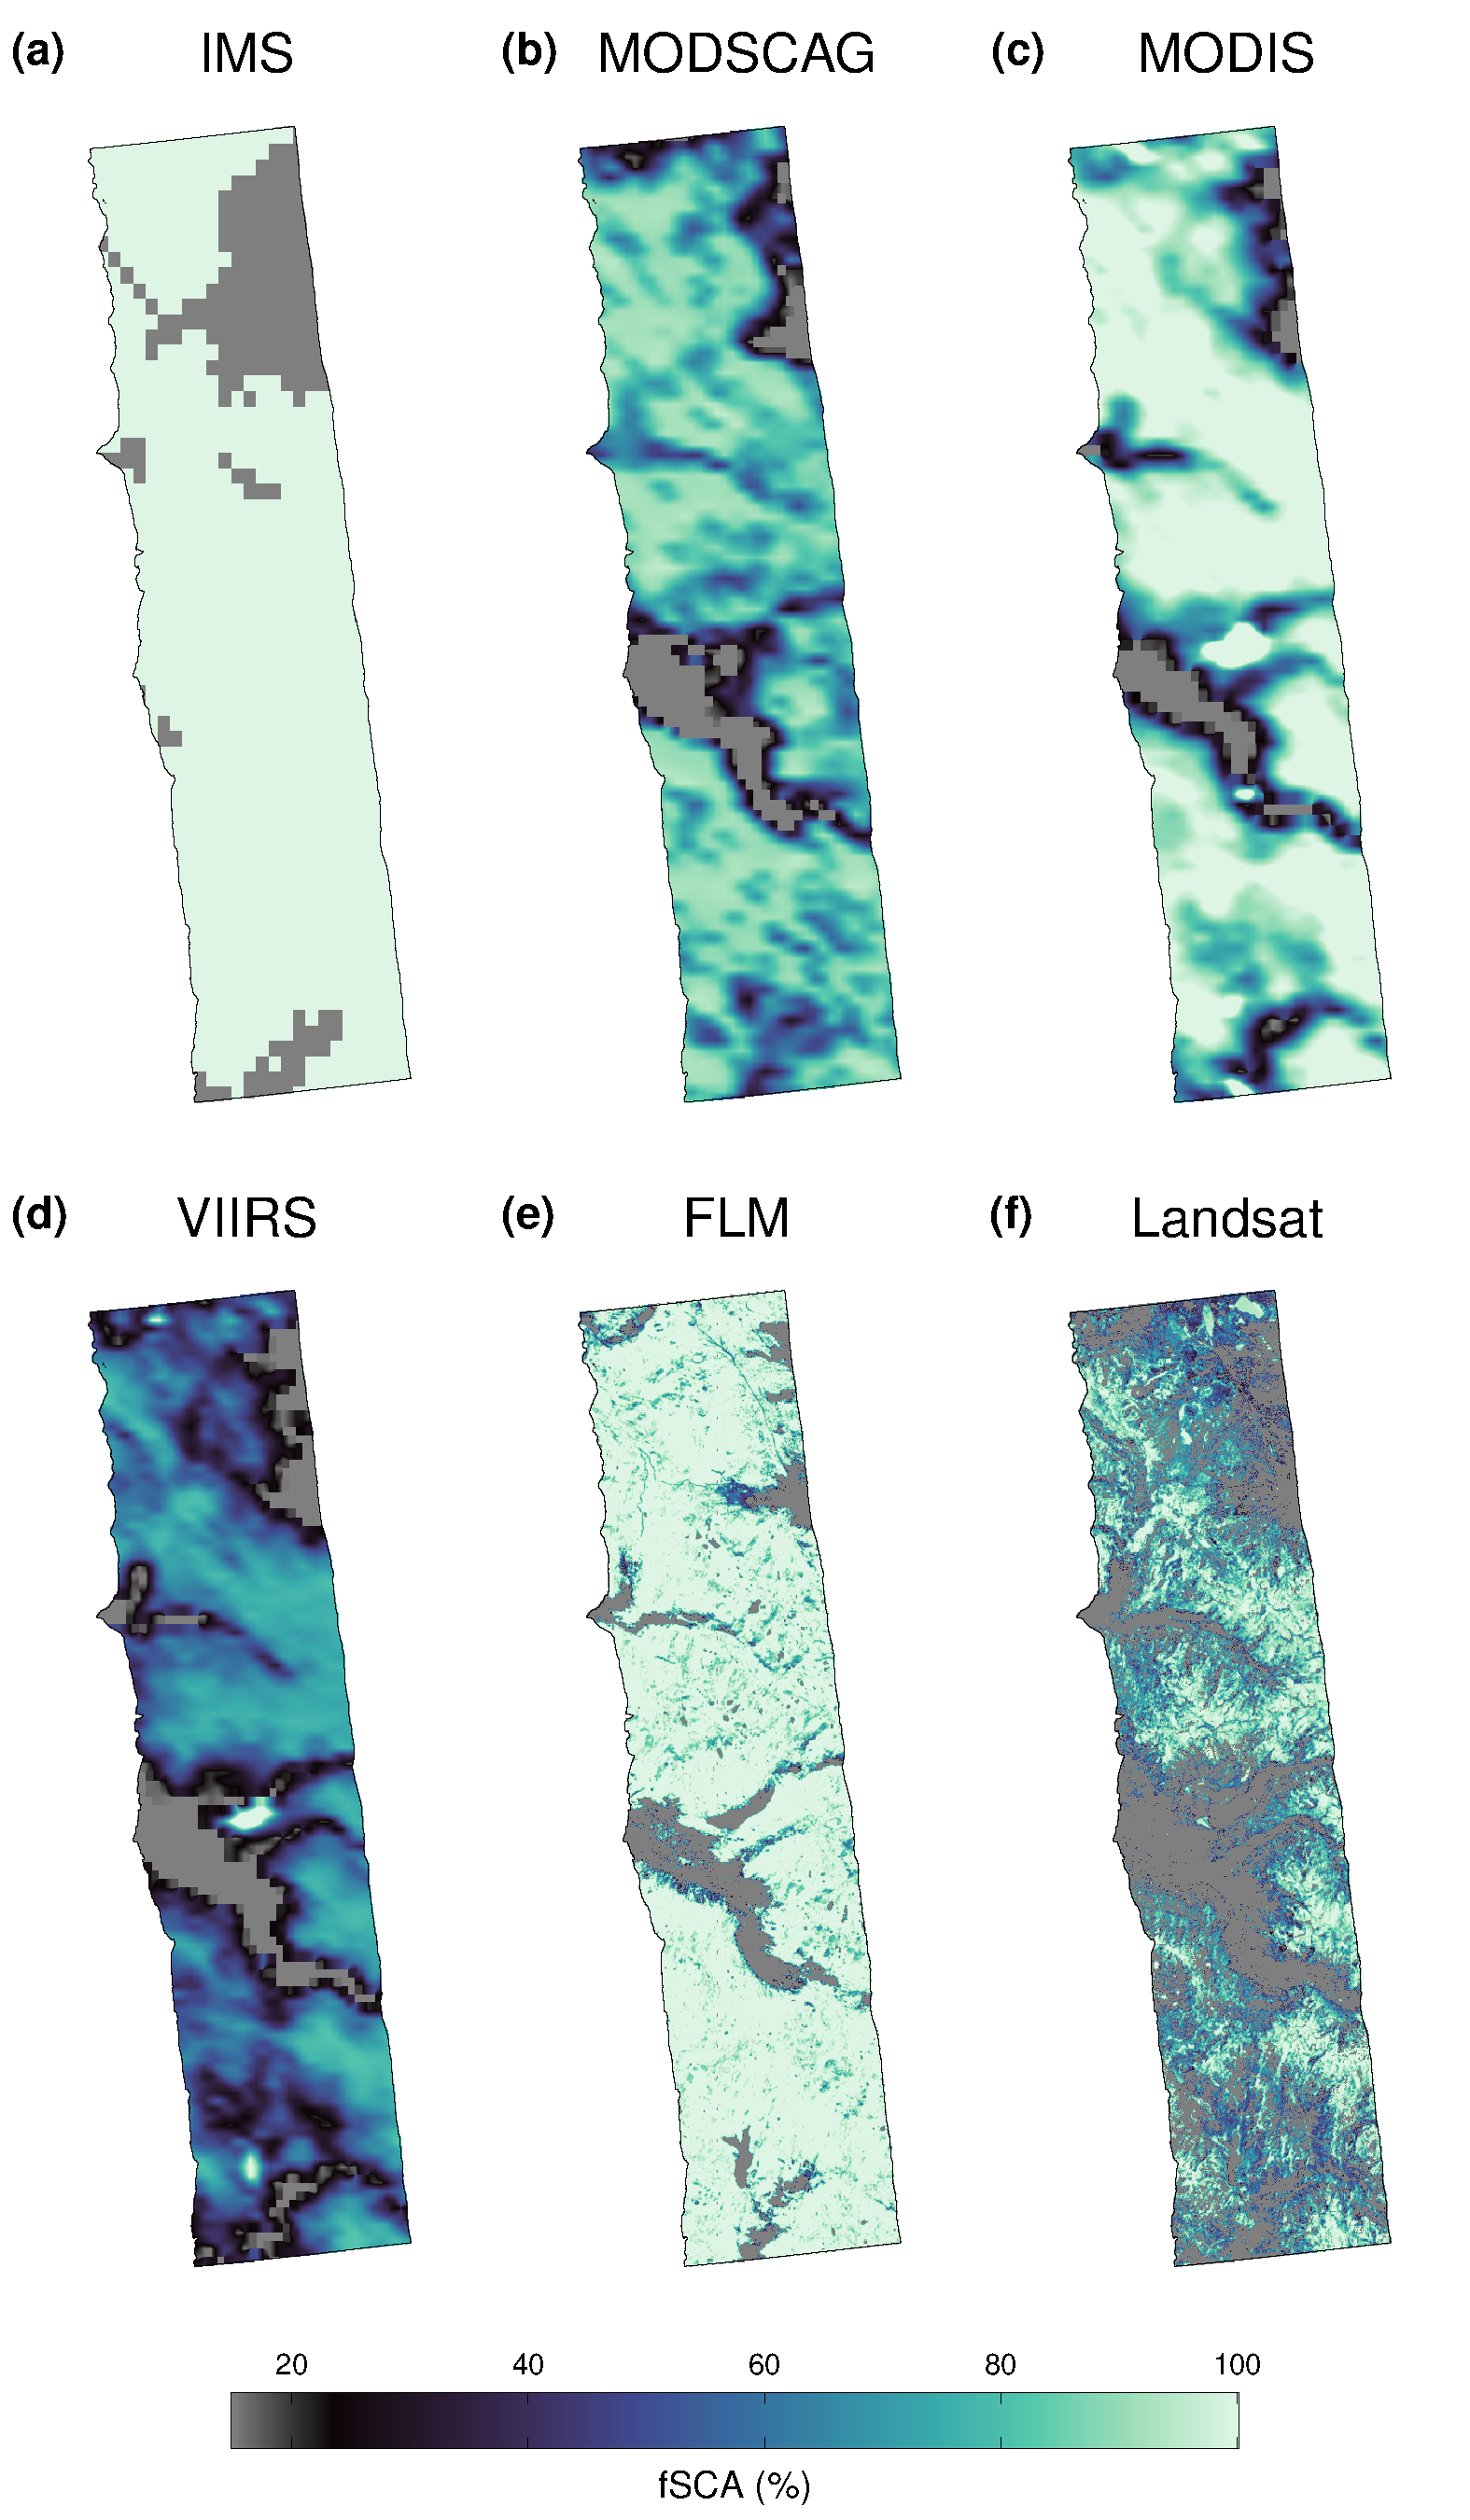
\includegraphics[width=13cm]{figures/ch4_figs/fsca_usvar_v2.pdf}
\caption{Snow cover data from \textbf{(a)} IMS, \textbf{(b)} MODSCAG, \textbf{(c)} MODIS fSCA, \textbf{(d)} VIIRS fSCA, \textbf{(e)} FLM, and \textbf{(f)} Landsat fSCA. The dark gray represents areas with <~15~\% fSCA}
\label{fig:fsca_plot}
\end{figure}

\clearpage
%%%%%%%%%%%%%%%%%%%%%%%%%%%%%%%%%%%%%%%%%%%%%%%%%%%%%%%%%%%%%%%%%%%%%%%%%%%%%%%%
\hypertarget{ch4-methods-3}{\subsubsection{IMS}\label{ch4-methods-3}}

The National Oceanic and Atmospheric Administration’s National Environmental Satellite Data and Information Service (NOAA/NESDIS) Interactive Multisensor Snow and Ice Mapping System (IMS) is a hemispherical scale binary 1 km snow cover product (Fig.~\ref{fig:fsca_plot}a) originally created to help with numerical weather prediction 
\citep{ramsayInteractiveMultisensorSnow1998, helfrichEnhancementsForthcomingDevelopments2007}. The input data come from a variety of platforms, including but not limited to: the National Oceanic and Atmospheric Administration's (NOAA's) next generation of geostationary satellites (GOES) constellation \citep{menzelIntroducingGOESIFirst1994}, the Advanced Very High Resolution Radiometer (AVHRR) \citep{cracknellAdvancedVeryHigh1997}, MODIS \citep{salomonsonMODISAdvancedFacility1989}, and the National Operational Hydrologic Remote Sensing Center (NOHRSC) SNOw Data Assimilation System (SNODAS) \citep{barrettNationalOperationalHydrologic2003}.

%%%%%%%%%%%%%%%%%%%%%%%%%%%%%%%%%%%%%%%%%%%%%%%%%%%%%%%%%%%%%%%%%%%%%%%%%%%%%%%%
\hypertarget{ch4-methods-4}{\subsubsection{MODSCAG}\label{ch4-methods-4}}

The MODIS Snow Covered Area and Grain size (MODSCAG) (Fig.~\ref{fig:fsca_plot}b) \citep{painterRetrievalSubpixelSnow2009} uses a spectral unmixing model that uses various end-members (e.g., rock, soil, snow, clouds, etc.) to produce estimates of fSCA, fractional vegetation (fVEG), snow grain size, and snow albedo at 500~m resolution.

%%%%%%%%%%%%%%%%%%%%%%%%%%%%%%%%%%%%%%%%%%%%%%%%%%%%%%%%%%%%%%%%%%%%%%%%%%%%%%%%
\hypertarget{ch4-methods-5}{\subsubsection{MODIS fSCA}\label{ch4-methods-5}}

The MODIS cloud-gap-filled (CGF) snow cover product \citep{hallEvaluationMODISVIIRS2019} provides daily NSDI values at 500~m spatial resolution from the Terra (MOD10A1F) and Aqua (MYD10A1F) satellites (Fig.~\ref{fig:fsca_plot}c). These data account for cloud cover by excluding pixels flagged as clouds and refilling them with NDSI from the last cloud-free day. This process only goes on for eight days of cloud cover until the pixel is marked as "no data" (NA). While questions remain about its efficacy \citep{nolinRecentAdvancesRemote2010, rittgerAssessmentMethodsMapping2013}, NDSI may be used to directly estimate fSCA \citep{salomonsonEstimatingFractionalSnow2004, salomonsonDevelopmentAquaMODIS2006,stillingerLandsatMODISVIIRS2023}. We computed the MODIS NDSI-based fSCA (herein, MODIS fSCA) using the Eq.~\ref{eq:fsca}:

\begin{equation}
\text{fSCA} = 0.01 + (1.45 \times NDSI)
\label{eq:fsca}
\end{equation}

\hypertarget{ch4-methods-6}{\subsubsection{VIIRS fSCA}\label{ch4-methods-6}}

The Visible Infrared Imaging Radiometer Suite (VIIRS) on the Suomi National Polar Partnership (S-NPP) produces a daily CGF NDSI product (VNP10A1F) at 375-m spatial resolution (Fig.~\ref{fig:fsca_plot}d) \citep{hallEvaluationMODISVIIRS2019}. These data are generated and gap-filled using the same methods as the MODIS CFG data outlined in Section \ref{ch4-methods-5}. We converted the VIIRS NSDI values to fCSA (herein, VIIRS fSCA) using Eq. \ref{eq:fsca}.

\hypertarget{ch4-methods-7}{\subsubsection{FLM}\label{ch4-methods-7}}

The fused Landsat-MODIS (FLM) (Fig.~\ref{fig:fsca_plot}e) fSCA product created by \cite{rittgerMultisensorFusionUsing2021} is spatiotemporally continuous 30~m over the Sierra Nevada, CA. The goal of their data fusion methods was to create a product with the high spatial resolution of Landsat (30~m) with the high temporal resolution of MODIS (1~d), leveraging the strengths of both sensors. These data were created using a combination of 170 Landsat scenes, daily MOD09GA Collection 6 in a sinusoidal projection at 463~m, physiographic information, spectral mixture algorithms, and random forest algorithm \citep{rittgerMultisensorFusionUsing2021}. 

\hypertarget{ch4-methods-8}{\subsubsection{Landsat fSCA}\label{ch4-methods-8}}

Landsat~8 fSCA (herein, Landsat fSCA) (Fig.~\ref{fig:fsca_plot}f) \citep{selkowitzUSGSLandsatSnow2017} data are generated using a spectral unmixing analysis based on the MODSCAG algorithm developed for MODIS \citep{painterRetrievalSubpixelSnow2009}. The data processing workflow includes water masking, cloud masking, and canopy cover corrections \citep{selkowitzUSGSLandsatSnow2017, stillingerLandsatMODISVIIRS2023}. The data products include both viewable fSCA and total ground fSCA. To estimate total fSCA in areas with canopy cover, a moving window analysis algorithm is employed.

\hypertarget{ch4-methods-8}{\subsection{In situ snow data}\label{ch4-methods-8}}

Snowpack information was collected at two pit locations in the UAVSAR Sierra flight line during the SnowEx 2020 campaign. One was dug near the US Army Corps of Engineers Cold Regions Research and Engineering Laboratory (CRREL) and the University of California, Santa Barbara (UCSB) joint “CUES” snow site study on Mammoth Mountain (37.6432533$^{\circ}$, $-$119.0290694$^{\circ}$) \citep{bairCUESStudySite2015}. The other was collected near Panorama Dome (37.6196618$^{\circ}$,$-$119.0002711$^{\circ}$). Snow density ($\rho_\mathrm{s}$) were measured in 10\,cm increments starting at the top of the pit. Unlike the in situ data used in \cite{tarriconeEstimatingSnowAccumulation2023a}, there were no direct values of permittivity measured during the data collection. We used snow pillow data from three snow pillows hosted on the California Data Exchange Center (CDEC): Volcanic Knob (VLC), Upper Burnt Corral (UBC), and Mammoth Pass (MHP). These data were used in the SWE change estimation to tether the relative InSAR data to a known change point.

\hypertarget{ch4-methods-9}{\subsubsection{Canopy Cover}\label{ch4-methods-9}}

For forest cover mapping, we used the National Land Cover Database (NLCD) \citep{homerConterminousUnitedStates2020} canopy cover data. These data are Landsat-based 30-m spatial resolution products that report land cover type and canopy cover percentage. These data are also used in the Landsat fSCA canopy cover correction.

%=============================================================================
%=============================================================================
%=============================================================================
\hypertarget{ch4-methods}{\section{Methods}\label{ch4-methods}}
\hypertarget{ch4-methods-1}{\subsection{Calculating InSAR $\Delta$SWE}\label{ch4-methods-1}}

First, the UAVSAR phase data were masked with each of the six fSCA products. A threshold of $>$\,15\,\% fSCA was set for a pixel to be considered snow covered. We then employ the InSAR $\Delta$SWE methodology described in Sec.~\ref{ch3-methods-1}. The SnowEx in situ data collection within the Sierra Nevada flight line did not include a permittivity measurement. Therefore, permittivity was estimated using the snow density-to-permittivity equation from \cite{guneriussenInSAREstimationChanges2001}:

\begin{equation}
\epsilon_\mathrm{s} = 1 + 1.6 * \rho_\mathrm{s} + 1.8 * \rho_\mathrm{s}^3
\label{eq:dens_to_perm}
\end{equation}

\noindent where snow permittivity is $\epsilon_\mathrm{s}$ and snow density is $\rho_\mathrm{s}$. Using Eq.~\ref{eq:insar_dswe}, pixel-wise $\Delta$SWE values were calculated with inputs of $\lambda$ (23.84\,cm), spatially distributed phase and $\theta$, $\rho_\mathrm{s}$ of 370~kg\,m$^{-3}$, and $\epsilon_\mathrm{s}$ of 1.68. 

To find the known change point to tether the initial relative InSAR $\Delta$SWE values, we used three snow pillows (VLC, MPH, UBC). The SnowEx $\Delta$SWE pit data could not be directly utilized as the phase values over the Mammoth CUES pit did not unwrap properly, resulting in the absence of any data. Additionally, the Panorama Dome pit was not dug during the study period. To account for uncertainties within the snow pillow geolocation, we extracted the UAVSAR pixel that the snow pillow was within and the eight surrounding pixels. We then took a spatial average of the relative InSAR $\Delta$SWE and the three pillows $\Delta$SWE values and subtracted them to obtain an absolute change. We report our volumetric $\Delta$SWE results in units of cubic decameters (dam$^{3}$). A cubic decameter is equal to 1000~m$^{3}$ or $\sim$0.81~acre-feet.

%==============================================================================
%==============================================================================
%==============================================================================
\hypertarget{ch4-methods-2}{\subsection{Quantifying $\Delta$SWE Variability}\label{ch4-methods-1}}

To understand how the various fSCA products impacted the scene wide $\Delta$SWE estimates, we performed a summing moving window analysis of the six UAVSAR-derived $\Delta$SWE datasets. The variability in the $\Delta$SWE data products solely comes from which pixels are considered snow covered and which are not. Therefore, a pixel-wise analysis is not an apt solution, as this would be comparing pixels with data to  NA (not available) values.

For the analysis, the $\Delta$SWE data were separated loss and gains to prevent the cancellation of patterns caused by opposite signs within an area. The pixel-wise SWE changes were then summed using a 41~$\times$~41 pixel moving window. The window size was subjectively selected based on exploratory analyses. Next, the standard deviation (SD) of the six moving window summed products was calculated. The relatively large window size was selected to minimize the occurrence of NA pixels in the SD calculation, where only datasets with 41-pixel squared areas of no snow will produce NA values. Summed pixels with NA values were not included in the SD calculations. We note that the northeast corner of the IMS data has a large region of NA values.

\hypertarget{ch4-results}{\section{Results}\label{ch4-results}}
\hypertarget{ch4-results}{\subsection{$\Delta$SWE Estimates}\label{ch4-results}}

The spatially distributed 80-m UAVSAR $\Delta$SWE estimates for each of the six fSCA products are shown in Fig.~\ref{fig:uavsar_dswe}. The black areas represent pixels removed in the unwrapping process (Fig. \ref{fig:uavsar_cor_inc_phase_plot}b), and are static throughout Fig.~\ref{fig:uavsar_dswe}a--e. The gray area represents pixels not considered snow covered by the given fSCA product, and these areas are spatially variable in the six scenes. Overall, the six scenes show a mean net SWE of $-$14,600~dam$^{3}$, with a mean gain of 3,100~dm$^{3}$ and loss of $-$17,800~dam$^{3}$ (Table~\ref{tab:dswe_stats}, Fig.~\ref{fig:dswe_bar_graph}). These values are consistent with in situ snow pillow data from this region, as there was a prolonged dry spell during 26 February to March 4 time span.

\clearpage
\begin{figure}[t]
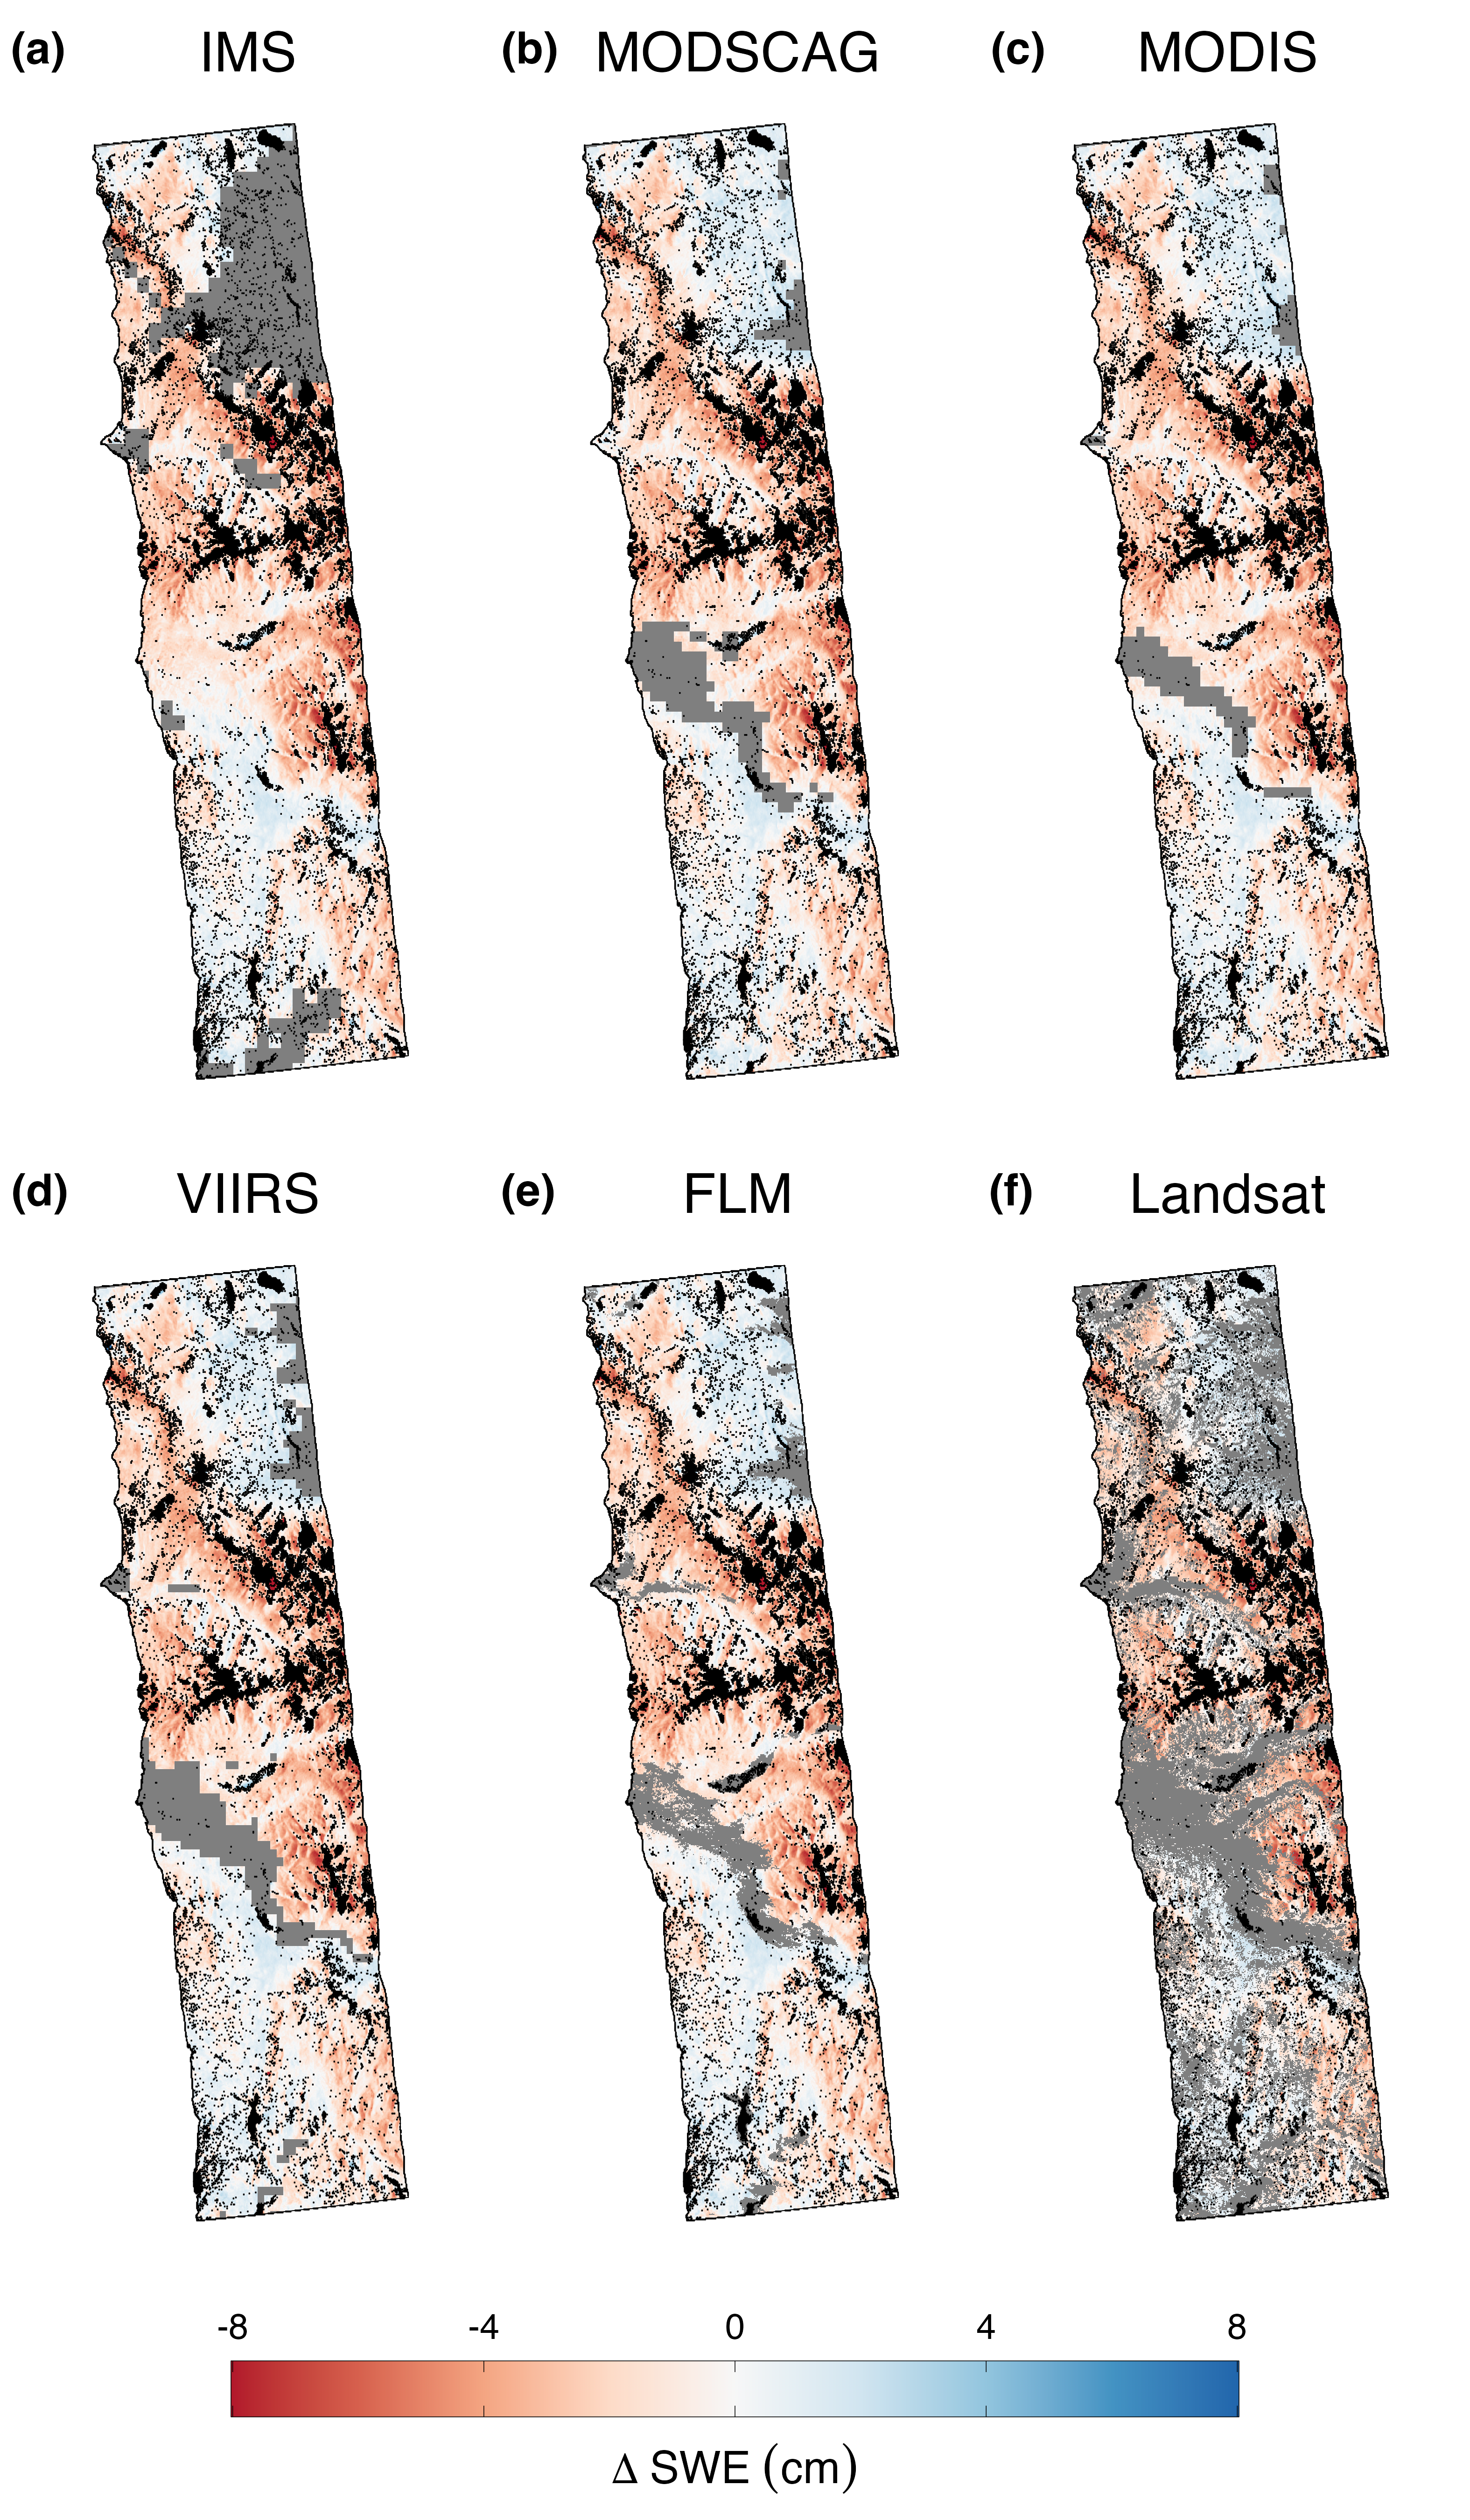
\includegraphics[width=\textwidth]{figures/ch4_figs/dswe_uavsar_v2.png}
\centering
\caption{UAVSAR InSAR derived $\Delta$SWE estimates with snow cover data from \textbf{(a)} IMS, \textbf{(b)} MODSCAG, \textbf{(c)} MODIS fSCA, \textbf{(d)} VIIRS fSCA, \textbf{(e)} FLM, and \textbf{(f)} Landsat fSCA. The dark gray represents areas with < 15 \% fSCA and the black represents pixels lost in the unwrapping process.}
\label{fig:uavsar_dswe}
\end{figure}

\clearpage
When disaggregated SWE gains vs. SWE losses, MODIS fSCA results shows the greatest SWE gain of 3,800~dam$^{3}$. The Landsat fSCA results show the least (2,100~dam$^{3}$) with the IMS showing a similar low value of 2,300~dam$^{3}$. The SWE gain values from MODSCAG, VIIRS fSCA, and FLM were quite similar to MODIS fSCA, with no product differing more than 400~dam$^{3}$.
MODIS fSCA also produced the greatest SWE loss ($-$19,100~dam$^{3}$), with Landsat fSCA again providing a low value of $-$12,900~dam$^{3}$. IMS, MODSCAG, VIIRS fSCA, and FLM again provided consistent estimates, with the standard deviation of these five data products' SWE loss being only 350~dam$^{3}$. Landsat fSCA's SWE loss of $-$12,900~dam$^{3}$ is $-$5,800~dam$^{3}$ greater compared to the five other data products mean SWE loss of $-$18,700~dam$^{3}$ (Fig.~\ref{fig:dswe_bar_graph}). These differences propagate into the net $\Delta$SWE values, where the five products other than Landsat fSCA provided highly consistent values, with a mean net $\Delta$SWE $-$15,400~$\pm$~300~dam$^{3}$. We report a 35.1~\% difference between the aforementioned mean value and Landsat fSCA.


\begin{figure}[]
\centering
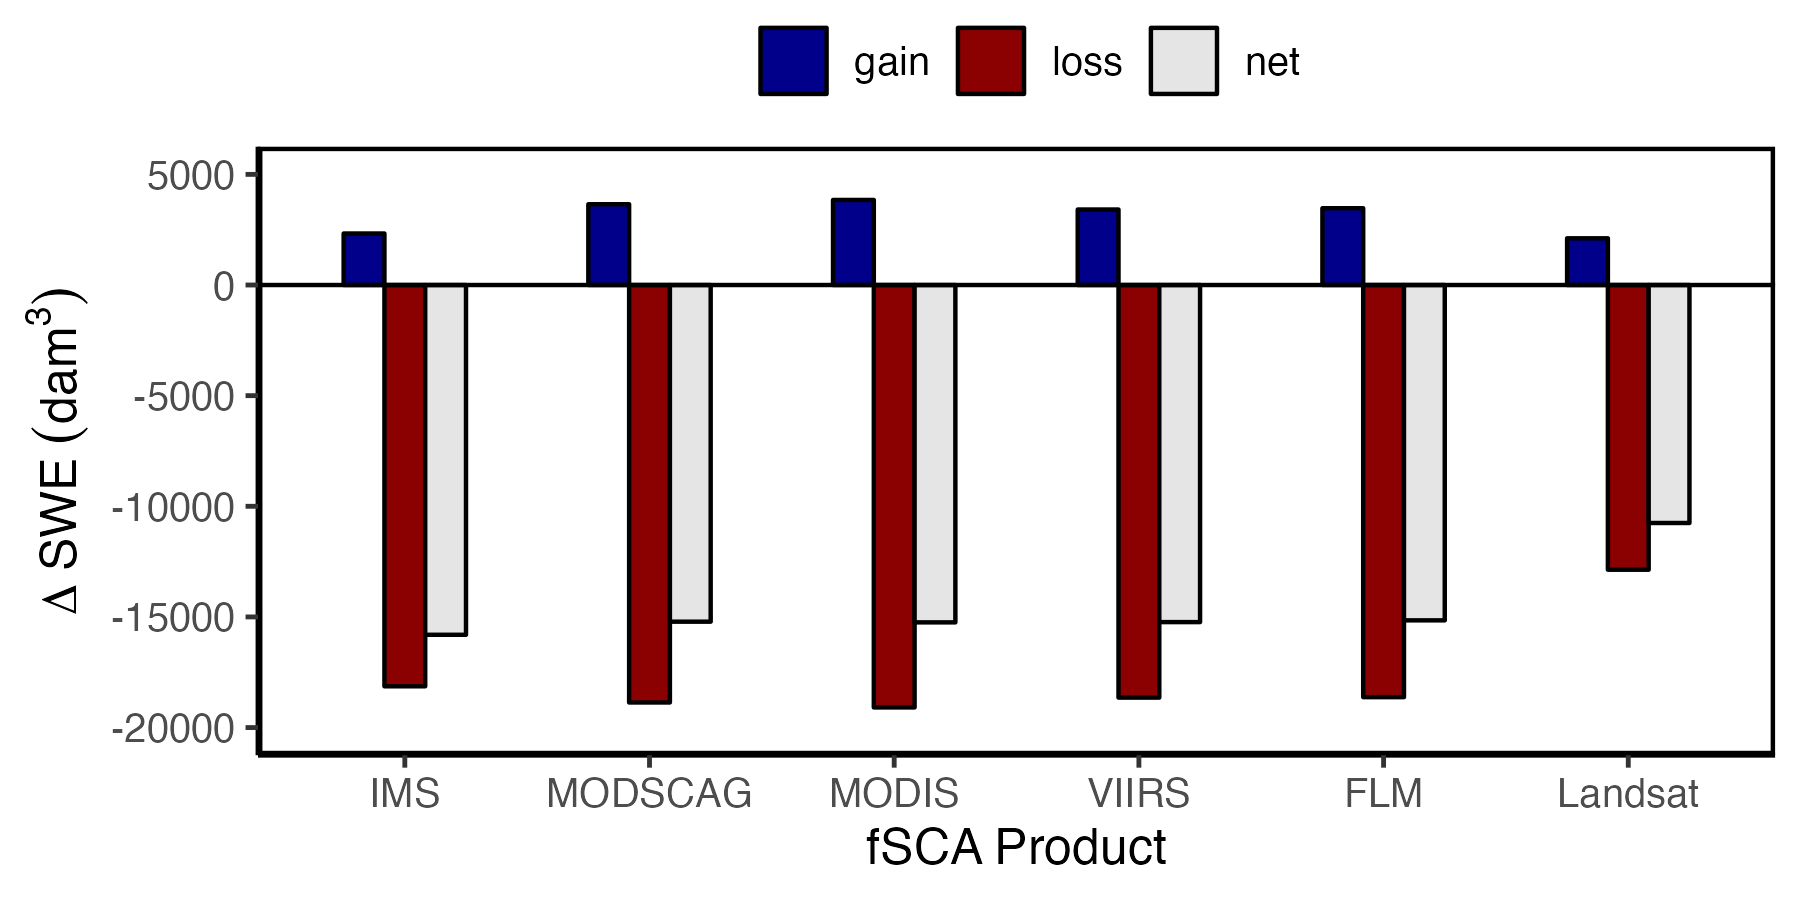
\includegraphics[width=\textwidth]{figures/ch4_figs/dswe_stats_dam3_v1.png}
\caption{Barplots of SWE gain, loss, and the net value for the six different snow cover products.}
\label{fig:dswe_bar_graph}
\end{figure}

\begin{table}
\centering
\caption{Displaying the total sum of $\Delta$SWE gains, losses, and overall net rounded to the nearest hundred for the six different snow cover products in Fig~\ref{fig:uavsar_dswe}.}
\begin{tabular}{lccc}
\toprule
& \multicolumn{3}{c}{$\Delta$SWE (dam$^{3}$)} \\
\midrule
fSCA Data & Gain & Loss & Net \\
\midrule
IMS & 2,300 & $-$18,200 & $-$15,900 \\
MODSCAG & 3,600 & $-$18,900 & $-$15,300 \\
MODIS fSCA & 3,800 & $-$19,100 & $-$15,300 \\
VIIRS fSCA & 3,400 & $-$18,700 & $-$15,300 \\
FLM & 3,400 & $-$18,700 & $-$15,200 \\
Landsat fSCA & 2,100 & $-$12,900 & $-$10,800 \\
\midrule
Mean & 3,100 & $-$17,800 & $-$14,600 \\
\bottomrule
\label{tab:dswe_stats}
\end{tabular}
\end{table}



\hypertarget{ch4-results}{\subsection{$\Delta$SWE Variability}\label{ch4-results}}

Fig.~\ref{fig:dswe_moving_window} shows the moving window sums of the $\Delta$SWE gains and losses. The majority of the SWE gains are recorded in the northeast and southeast portions of the swath. The SWE gain spatial patterns between the datasets are similar except for the northeast corner of the IMS data. This area is shown as no snow while MODSCAG, MODIS fSCA, VIIRS fSCA, and FLM display SWE gains on the order of 100--150~dam$^{3}$. Landsat fSCA shows SWE gain in this area as well but with a lesser magnitude of $\sim$50~dam$^{3}$. All datasets other than Landsat fSCA show consistent spatial patterns and SWE loss magnitudes. Landsat fSCA's spatial patterns are similar but with a lower amount of $\Delta$SWE. This is driven by Landsat fSCA data not being as spatially continuous. The large area of NA values in the IMS data is not of concern as this was an area of slight SWE gain. In the center left of the swath, all datasets show a lower elevation snow free area except for IMS. However, most of the $\Delta$SWE values in that area and relatively small, therefore, do not significantly bias the results.

The 41 $\times$ 41 moving window pixel-wise SD of SWE gains and losses are compared to canopy cover percentage in Fig.~\ref{fig:dswe_standard_deviation}. For SWE gains, the area with the greatest SD (30--50~dam$^{3}$) was in the northeast corner of the swath. The sharp transition from red to green is driven by the NA values in the IMS data. Large SWE loss variability was centered around the lower elevation area in the middle of the scene. These SWE loss SD values show similar spatial patterns to that of the canopy cover data in Fig.~\ref{fig:dswe_standard_deviation}c. $\Delta$SWE SD is directly compared to canopy cover percent in Fig.~\ref{fig:dswe_boxplots}. Generally, the SD for SWE gains and SWE losses increases as canopy cover increases, yet there is variability in the relationship.

\clearpage
\begin{figure}[h]
\centering
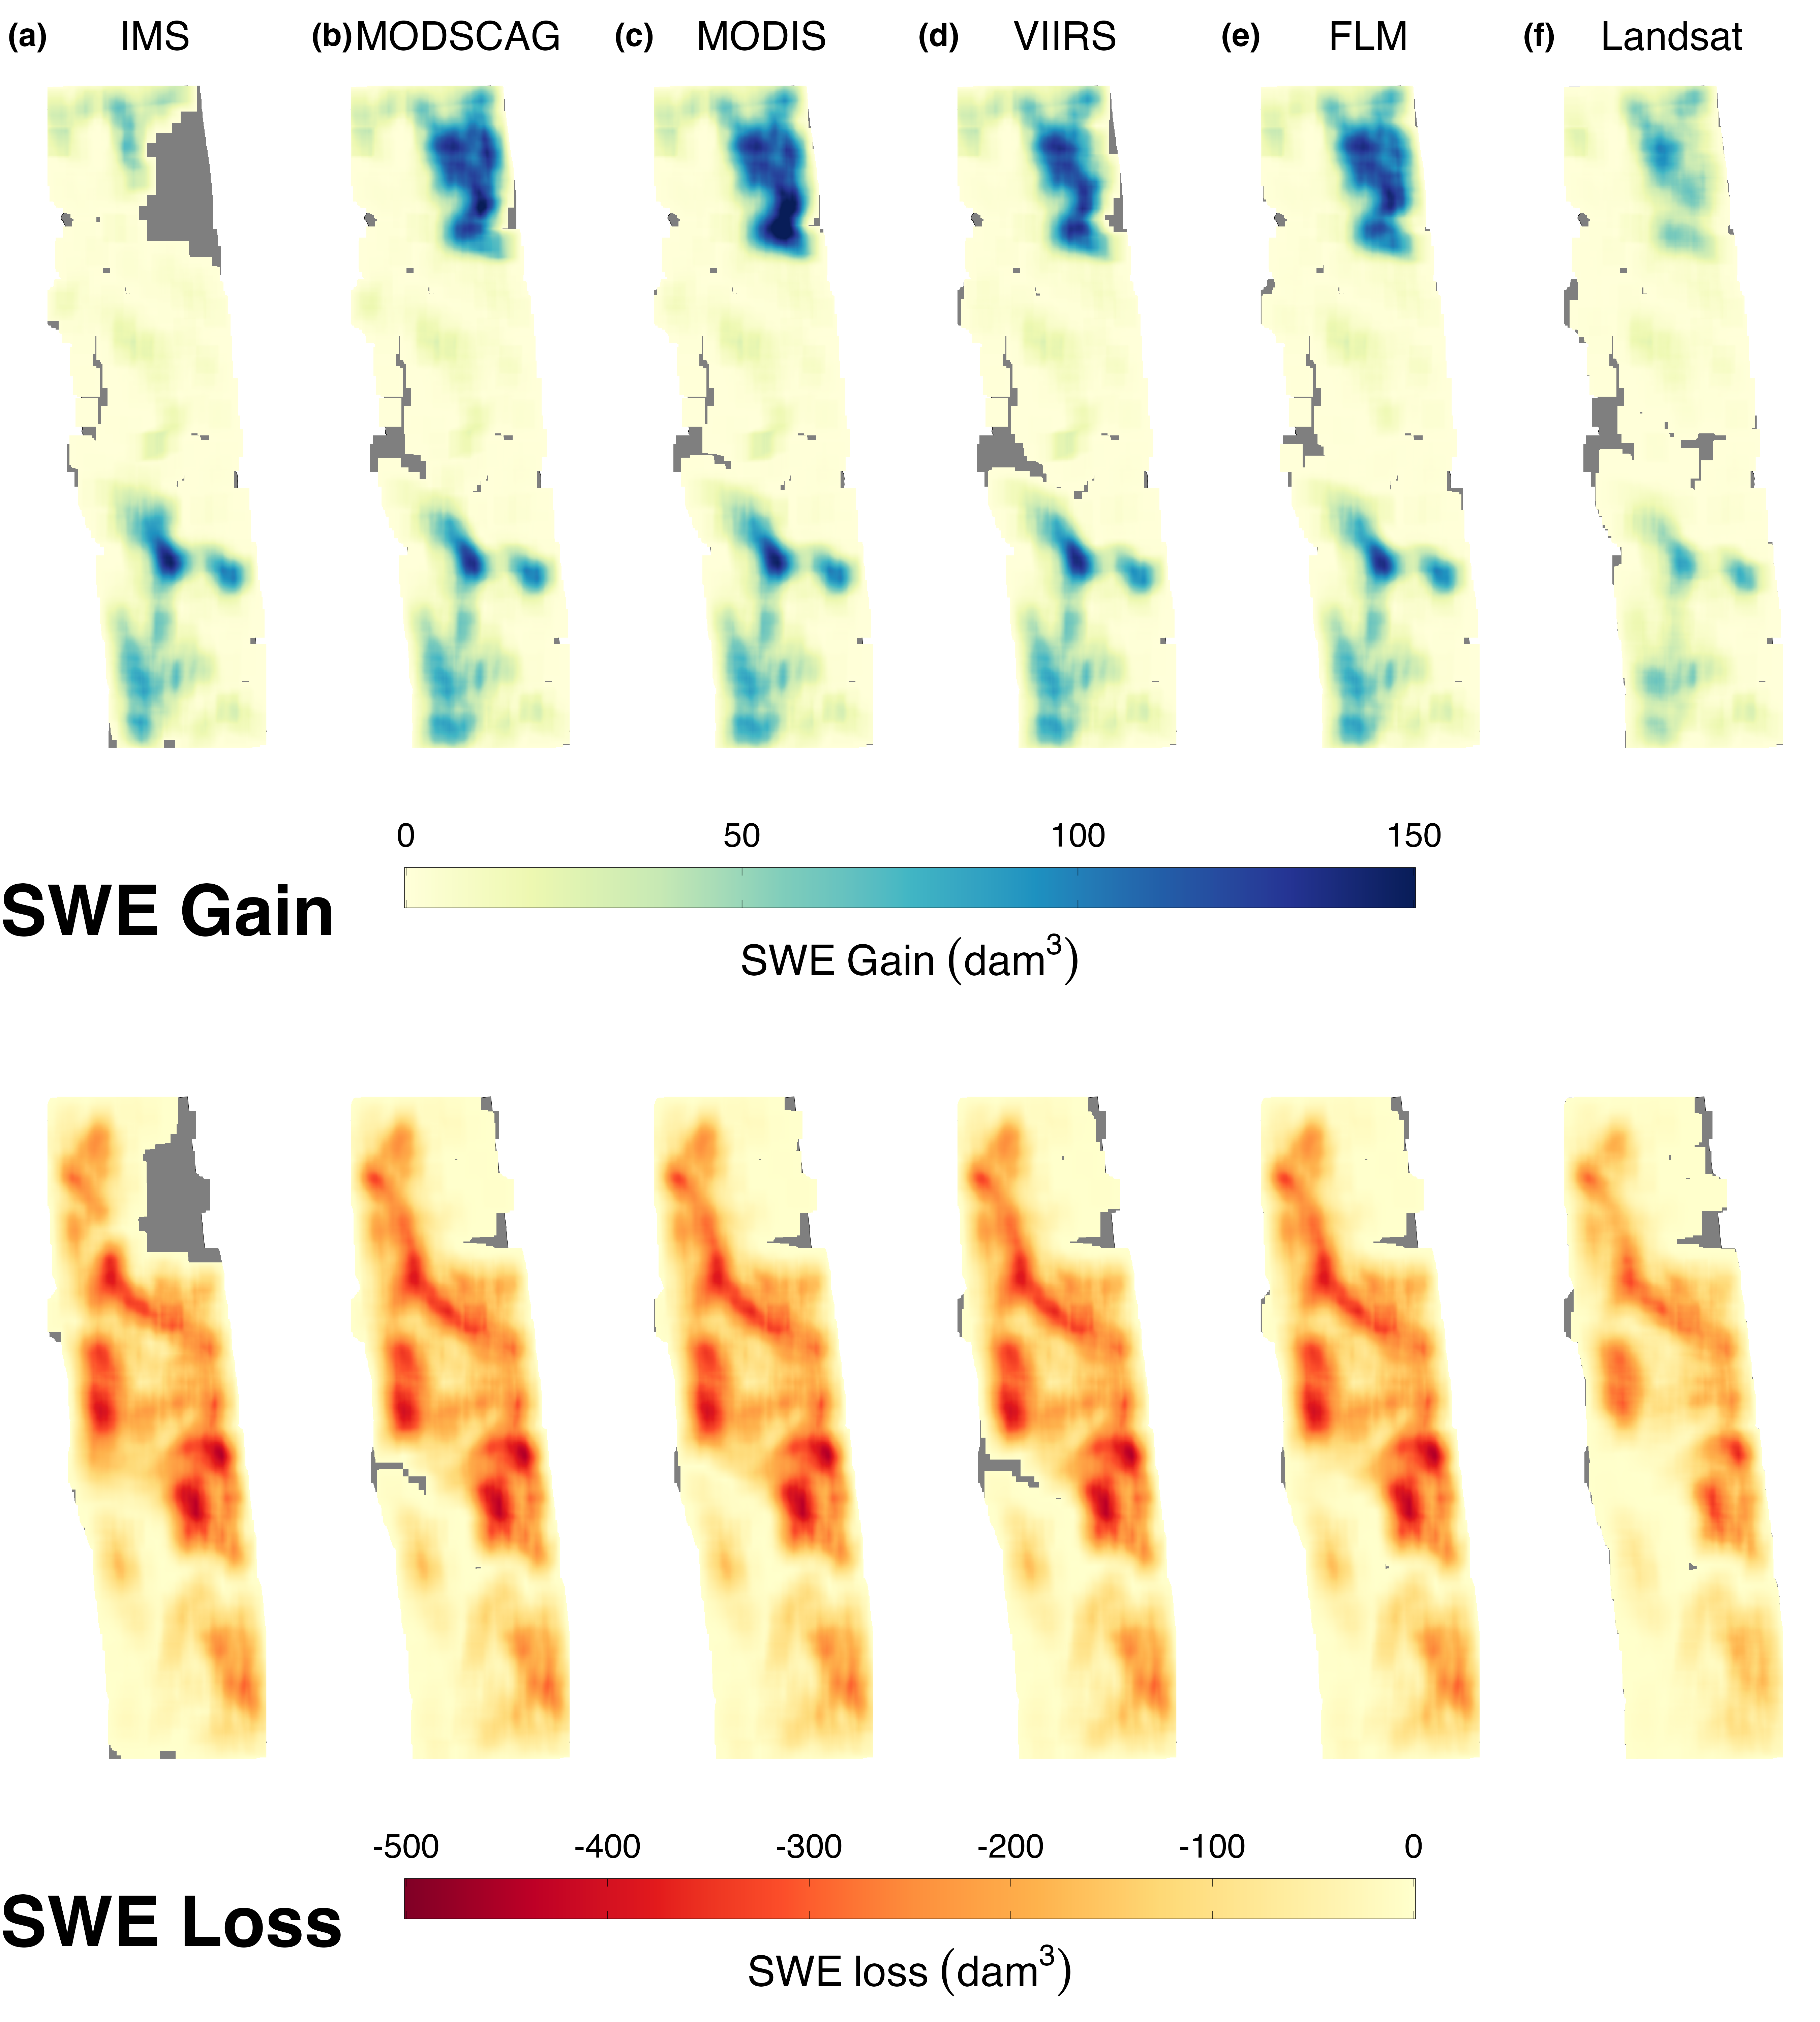
\includegraphics[width=\textwidth]{figures/ch4_figs/dswe_mw_full_dam3_v1.png}
\caption{$\Delta$SWE moving window analysis for SWE gains (top) and SWE losses (bottom) for the six different $\Delta$SWE products.}
\label{fig:dswe_moving_window}
\end{figure}


\clearpage
\begin{figure}[t]
\centering
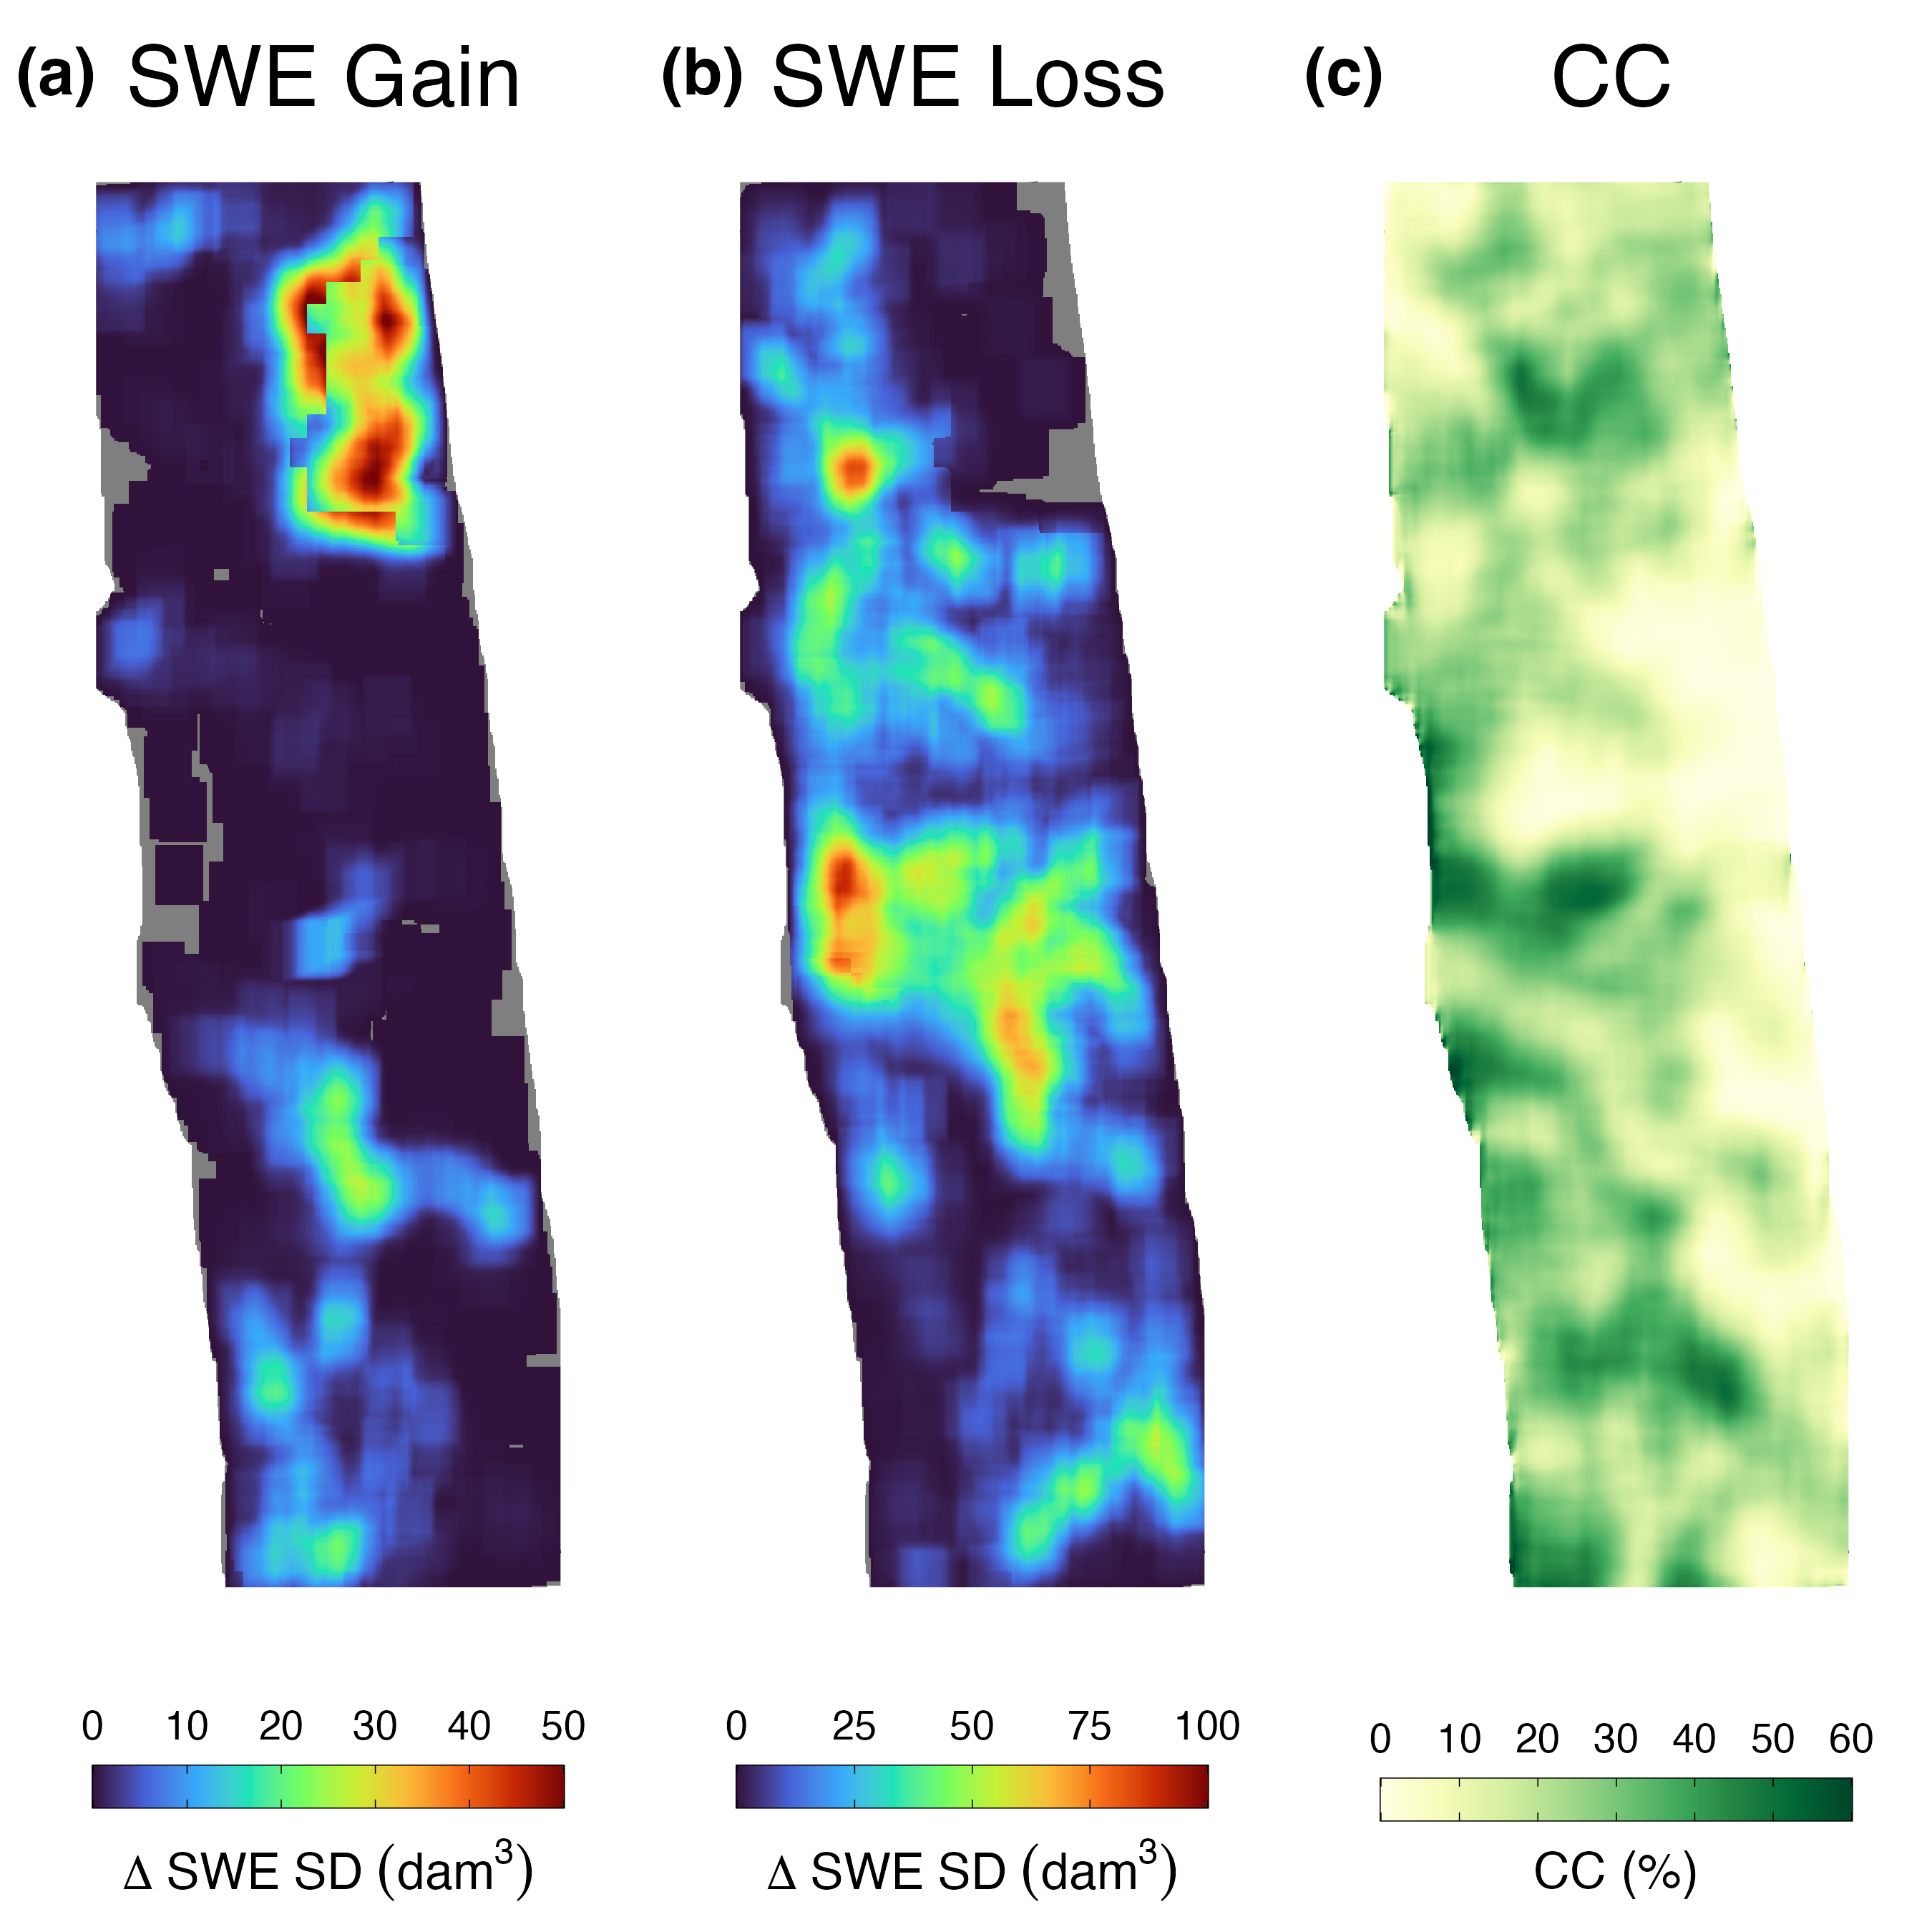
\includegraphics[width=\textwidth]{figures/ch4_figs/sd_vs_cc_map_dam3_41x41_v2.png}
\caption{howing SD \textbf{(a)} SWE gain and \textbf{(b)} SWE Loss between the six a 41~$\times$~41 pixel moving window $\Delta$SWE estimates. \textbf{(c)} The moving window canopy cover percentage.}
\label{fig:dswe_standard_deviation}
\end{figure}

\clearpage
\begin{figure}[t]
\centering
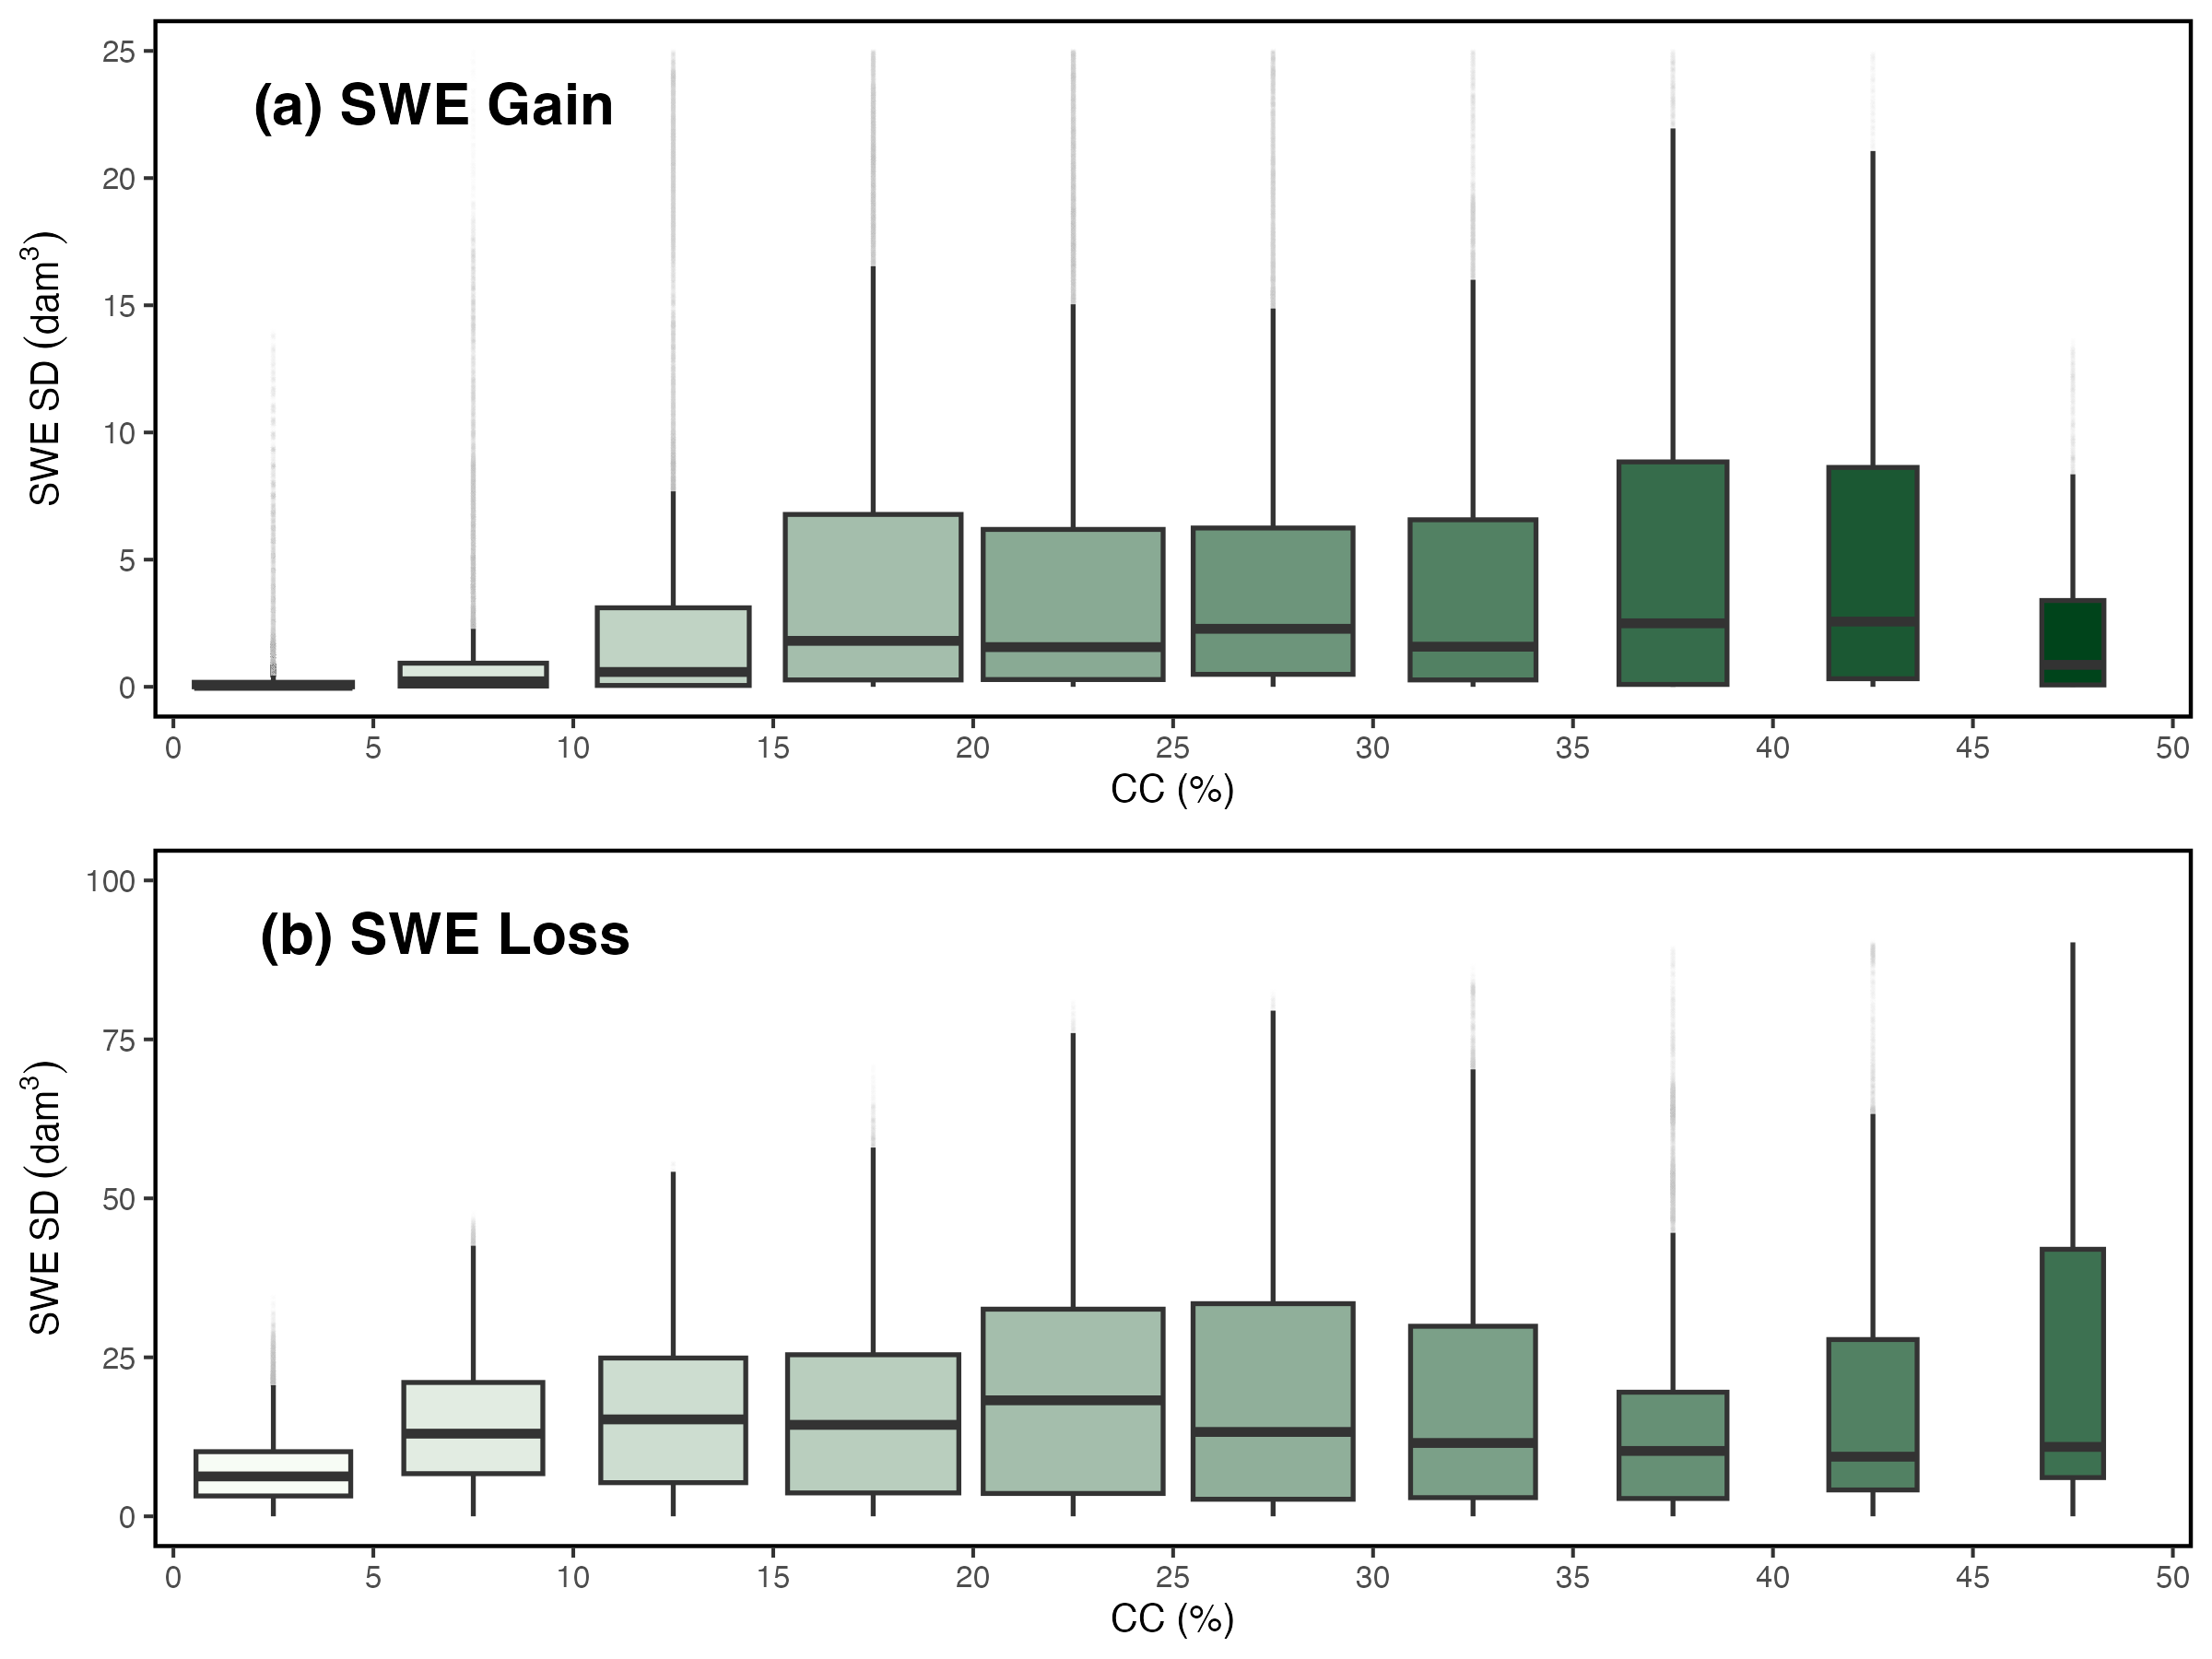
\includegraphics[width=\textwidth]{figures/ch4_figs/swe_sd_bp_dam3_41x41_v1.png}
\caption{Boxplots showing the relationship between CC \% and SWE SD for \textbf{(a)} gain and \textbf{(b)} loss. The y-axis is set individually for each plot for data visualization purposes.}
\label{fig:dswe_boxplots}
\end{figure}

%==============================================================================
%==============================================================================
%==============================================================================
\hypertarget{ch5-discussion}{\section{Discussion}\label{ch4-discussion}}
\hypertarget{ch5-discussion-1}{\subsection{Key findings and future directions}\label{ch4-discussion}}

We originally hypothesized that a daily, high spatial resolution fSCA product such as FLM would provide the most realistic results as it uses information from both Landsat and MODIS. Surprisingly, the coarse spatial resolutions of MODIS fSCA/MODSCAG (500~m), and VIIRS fSCA (375~m) which create an imprecise representation of the snowline, don't significantly impact the overall $\Delta$SWE results when compared to FLM. \cite{stillingerLandsatMODISVIIRS2023} performed an uncertainty analysis of various fSCA products from MODIS, VIIRS, and Landsat using airborne lidar-based fSCA as validation. They found some variability in the fSCA products, with the spectrally unmixed data performing better, but overall modest differences. It is promising that fSCA derived from MODIS and VIIRS NDSI data, currently produced in near-real-time by NSIDC, can generate fSCA estimates for SAR-based SWE retrievals that yield nearly identical values (Table~\ref{tab:dswe_stats}) to that of the more complex spectral unmixing and machine learning methods employed by MODSCAG and FLM. Additionally, these products are not currently hosted openly on a NASA DAAC. This means that upon the launch of NISAR in early 2024, the moderate-resolution sensor can provide a reasonable snow cover boundary for basin-scale water resource applications. 

While there were broad similarities, our results show that significant InSAR-based $\Delta$SWE estimation variability can arise from fSCA product choice. The variability in how snow cover is defined arises from two main sources: primarily, sub-canopy snow cover estimation methodology, and secondarily, native product spatial resolution. The five fSCA products, excluding Landsat fSCA, showed broad similarities in their fSCA estimation in forest areas. For the coarser resolution products (MODIS fSCA, VIIRS fSCA, and IMS), the larger pixel size has more sub-pixel variably, with fewer pixels having less than 15~\% fSCA. For the finer-resolution products (FLM and Landsat fSCA), their main differences arise from the sub-canopy fSCA estimation. 

The Landsat fSCA data had the greatest variability in fSCA across the study area, which then propagated into SWE gains and losses of lesser magnitude when compared to the other five products. These losses are driven by how the Landsat fSCA data estimate sub-canopy snow cover. They use a multi-step moving window canopy adjustment. It employs a 11~$\times$~11 and a 31~$\times$~31 moving window to infill surrounding pixels depending on canopy cover percentage, elevation, cloud cover, and incoming solar radiation \citep{selkowitzUSGSLandsatSnow2017}. If a pixel is >~60~\% canopy cover, it is automatically excluded from snow cover eligibility. We hypothesize that the dense conifer forest in parts of the UAVSAR study area, with 48~\% of the total forest having a canopy cover density of >~40~\%, created conditions where the algorithm didn't detect sub-canopy snow cover. The second source of uncertainty stems from the pixel size. Pixel size changes the calculated amount of land within the study area \citep{bairHowTradeoffsSatellite2023}. Here, we see that both the study area size and the SCA precision are affected by the native product resolution. This impacts the snow line estimates yet was of lesser concern when compared to the canopy cover considerations.

%%% thoughts on fSCA and forests
It is important to note that fSCA data have not traditionally been used in combination with radar data for SWE estimation. Past SWE estimation efforts have implemented fSCA in combination with a spatially distributed energy balance model to derive SWE in various reconstruction approaches \citep{clineEstimatingSpatialDistribution1998,molotchEstimatingDistributionSnow2008,rittgerSpatialEstimatesSnow2016,margulisLandsatEraSierraNevada2016}. Because this is a first effort in to estimate SWE using radar and optically-derived SCA, we set a lower threshold for fSCA in our study areas. For this, we employed a 15\% fSCA threshold to determine the inclusion of pixels as snow covered. This subjective choice was based on the minimum threshold set in \cite{painterRetrievalSubpixelSnow2009}. 

% future work with forests
While not the main focus of this study, future work should focus on the uncertainties associated with all SAR-based SWE retrieval techniques with respect to fSCA and canopy cover. Whether it is the InSAR phase-based technique presented here with L-band, P-band \citep{shahRemoteSensingSnow2017,maEstimatingSpatiotemporallyContinuous2023}, C-band \citep{lievensSnowDepthVariability2019,oveisgharanSnowWaterEquivalent2023}, or Ku-band \citep{tsangReviewArticleGlobal2022,rottColdRegionsHydrology2010}, all techniques will have to quantify the uncertainty associated with mixed pixels. As seen the in the Landsat fSCA data used in this study, very few 80~m square areas are completely snow covered. There are bare areas driven by prevailing wind patterns and aspect-based solar radiation variations, as well at large areas of the swath consistent conifer forest canopy. In the Cold Regions Hydrology High-Resolution Observatory (CoReH$_{2}$O) mission (Ku-band) developed by \cite{rottColdRegionsHydrology2010}, they note the importance of accounting for three-dimensional canopy structure on backscatter values. \cite{lemmetyinenAttenuationRadarSignal2022} showed radar signals at various wavelengths have different sensitives to forest canopy, with above-freezing temperatures increasing the uncertainty. Continuing to unravel the impacts of forests on SAR-based SWE retrievals from airborne and spaceborne platforms should be the topic of future investigations.

While we showed the moderate-resolution products are sufficient, future work should continue to focus on producing fSCA data products at finer spatial and temporal resolutions. This should in incorporation Very-High-Resolution (VHR) commercial satellite imagery \citep{huImprovingMountainSnow2022, thalerEstimatingSnowCover2023,yangHighresolutionMappingSnow2023,johnHighResolutionSnowCoveredArea2022}, as well as the Sentinel-2 constellation \citep{gascoinEstimatingFractionalSnow2020}.

%%%%%%%%%%%%%%%%%%%%%%%%%%%%%%%%%%%%%%%%%%%%%%%%%%%%%%%%%%%%%%%%%%%%%%%%
%%%%%%%%%%%%%%%%%%%%%%%%%%%%%%%%%%%%%%%%%%%%%%%%%%%%%%%%%%%%%%%%%%%%%%%%
%%%%%%%%%%%%%%%%%%%%%%%%%%%%%%%%%%%%%%%%%%%%%%%%%%%%%%%%%%%%%%%%%%%%%%%%
\hypertarget{ch5-discussion-2}{\subsection{Limitations}\label{ch4-discussion-2}}

% no truth, just variability
Our study did not aim to validate the given data products with respect to the validation dataset. Many past studies have used Landsat, with various spectral unmixing approaches, as their validation data set \citep{painterRetrievalSubpixelSnow2009,rittgerAssessmentMethodsMapping2013} or airborne lidar \citep{stillingerLandsatMODISVIIRS2023}. While it's impossible to confidently say whether or not a sub-canopy area is completely snow covered, we assume that the high-elevation parts of the USJ were snow covered. This suggests that Landsat fSCA was underestimating fSCA and $\Delta$SWE, as it had far greater amount of pixels considered NA. Our variability analysis was an imperfect comparison between the six data products. While we used a 41 $\times$ 41 moving window, the IMS data had a large continuous snow-free area in the northeast corner. These pixels were then omitted from the standard deviation analysis, propagating uncertainty in the calculation as one dataset was not used.

% study area and short time period
The UAVSAR flight line was over a high elevation (mean of 2733~m) portion of the USJ, where a majority of the swath was snow covered. Due to the small study area and high snow cover percentage, there was limited variability in the snow cover products. Addtionally, during the two-week study period, there were no large precipitation events, and therefore snow cover was relatively constant. In future satellite-based basin-scale analyses, there will be a greater range and variability of fSCA values, as well as more lower-elevation forest cover. Large atmospheric river-type storms in the Sierra can significantly shift the snow line. This presents challenges for the products that do not have a daily temporal resolution, such as Landsat. We chose to analyze data over a short study window (14~d) and therefore did not fully address the effects temporal resolution has on SWE change estimates. Future work should focus on the $\Delta$SWE uncertainties that come from infrequent fSCA data. We calculated the average SWE change between three snow pillows to identify the InSAR known change point. There was disagreement between the UAVSAR estimated SWE change and the in situ values, and this point to uncertainty in the unwrapping process and intra-swath atmospheric effects. As stated in \cite{tarriconeEstimatingSnowAccumulation2023a}, high accuracy near-real-time mountain range scale atmospheric correction is the main uncertainty facing InSAR SWE change monitoring. 

%=============================================================================
%=============================================================================
%=============================================================================
\hypertarget{ch6-conclusions}{\section{Conclusions}\label{ch6-conclusions}}

This study set out to understand how snow cover product selection impacts $\Delta$SWE estimates in a multisensor optical-radar approach. While we showed that there is variability between the snow cover products, there are broad similarities in the SWE retrievals. The key finding is that moderate-resolution NDSI-based SCA products can be effectively used in optical-radar SWE retrievals in mountain regions. We originally hypothesized that a 30~m product would be optimal for this multisensor approach, yet our results show that there is essentially no difference in SWE gains and SWE losses when comparing the FLM with other coarser snow cover products. This means that the widely available, moderate resolution (375--500~m) snow cover products will likely be sufficient for future multisensor optical-radar SWE retrievals. 

\clearpage
\bibliographystyle{apalike}
\setstretch{1}
\bibliography{ch4.bib}
\setstretch{1.5}
